\fancyhead[R]{Python Application Energy Consumption}
\section{Experiment Design}
\label{sec:experimentdesign}
The experiment design is illustrated in \autoref{fig:design}. The design consists of three main parts: a PC used to control the experiment, an RPi, and an Otii. The PC is connected to the Otii via USB cable for reading data, and to the local network via ethernet cable to allow SSH access to the RPi. The Otii is powered by a 25 volt power supply, and in turn powers the RPi via USB-C. The RPi is also connected to the local network via ethernet cable. The PC uses Otii 3 Software to control the power supply from Otii to RPi and record data.

\begin{figure}[H]
    \centering
    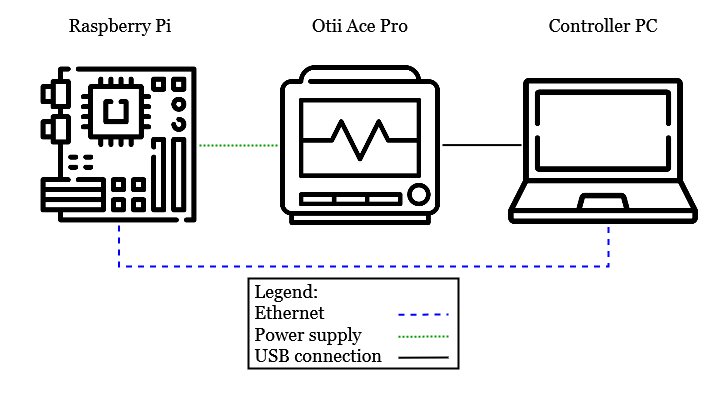
\includegraphics[width=0.7\textwidth]{images/experiment.png}
    \caption{Experiment design for measuring power draw, runtime and energy consumption of RPis during Python benchmark execution}
    \label{fig:design}
\end{figure}

SD cards with the four OSs and five Python versions installed are prepared beforehand. Pyperformance has also been individually installed for each version of Python, as is required to run benchmarks for a specific version. A large fan is set up to continually cool the RPi, and CPU temperature is then queried directly on the RPi through another SSH terminal on the PC, before, during, and after benchmarks. This is to make sure that rising CPU temperature doesn't skew the measurements for longer benchmarks, since CPUs are known to perform worse at higher temperatures\cite{benoit2020impact}. Throughout the entire benchmarking process, the CPU temperature never rises above 37$^{\circ}$C, which is deemed satisfactory for consistency of results. OSs are installed in their default configurations to make sure that any potential differences in energy consumption between them can be explained by the OS implementation specifics alone, and not by the quality of performance optimizations made by the user.

\begin{figure}[H]
    \centering
    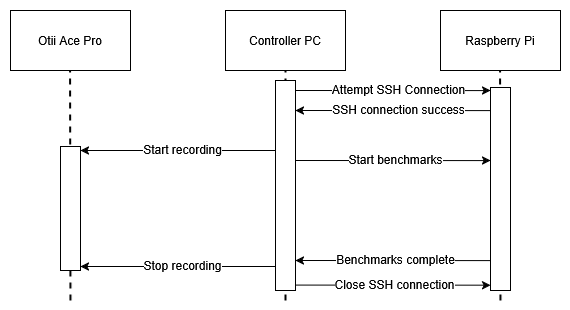
\includegraphics[width=0.8\textwidth]{images/thesis_sequence.png}
    \caption{High-level sequence diagram showing the sequence of actions involved in running the experiment}
    \label{fig:sequence}
\end{figure}

\autoref{fig:sequence} shows the actions involved in running the experiment, and how the three main devices interact with each other. On each RPi, the process shown is repeated ten times for each unique combination of Python version, OS, and RPi, totalling 400 recordings across 40 configurations. For detailed instructions on how to run the experiment, install the OSs and Pyperformance, open SSH sessions, and query temperature, see the repository.
